\section{Det samlede system}\label{sec:samlet_system}
\textit{Dette afsnit omhandler test af det samlede system, hvis design og implementering består af indholdet fra de forrige blokke. Designet af det samlede system har til formål at opfylde de specifikke krav i \secref{krav_samlet_sys}.}

Det samlede system består en række blokke, som tidligere er blevet designet, implementeret og testet for, hvorvidt disse blokke opfylder deres krav. Det fremgår af testene, at de separate blokke overholder de opstillede krav. Det samlede system sammensættes af hver enkelt blok og implementeres, som det fremgår af \figref{fig:design_blokdiagram}.% Det følgende afsnit vil derfor indebære en test af funktionaliteten for det samlede system i forhold til kravene opstillet i \secref{krav_samlet_sys}. 

\subsection{Test}
Testen udføres med henhold til de opstillede krav og tilhørende tilladte afvigelser opstillet i \secref{krav_samlet_sys}. Kravene beskriver, at det samlede system skal:
\begin{itemize}
	\item Kunne detektere aktiviteterne gang, løb og cykling ved brug af gyroskop og accelerometer. Der accepteres ikke brug af andre sensorer.
	\item Kunne lave automatisk adskillelse af gang, løb og cykling ved hjælp af algoritmer. Der accepteres en afvigelse på 10\% i forhold til fejlvurdering af aktivitet.
	\item Kunne detektere puls ved brug af pulssensor og tilhørende algoritme samt derefter kategorisere intensiteten af en given aktivitet. Der accepteres en pulsafvigelse på 10\%.
	\item Videresende signaler til en ekstern enhed ved hjælp af BLE. Der accepteres ikke andre trådløse kommunikationsformer.
	\item Besidde batterilevetid for en hel dag svarende til 15 timer. Der accepteres ikke en batterilevetid på mindre end 15 timer.
	\item Repræsentere varigheden og pointfordelingen af en given aktivitet i GUI. Der accepteres ikke en anden form for visualisering. 
\end{itemize}
Kravet om registrering af puls vil ikke blive opfyldt, da pulssensoren ikke indgår i det samlede system, se \secref{sec_de_im_te_puls}. Det første krav om brug af accelerometer og gyroskop er opfyldt, da disse sensorer netop er valgt til formålet. Derudover er systemet designet til at sende via BLE, og en GUI bliver anvendt til datavisualisering. Derved overholdes disse krav også på forhånd. \\
Formålet med test af det samlede system er altså at undersøge, hvorledes de resterende krav samt tolerancer overholdes. Det samlede systems funktionalitet testes ved først at opsætte softwaren på ICen og GAP peripheral ved hjælp af PSoC programmer. Derefter skal ICen sammensættes med MCUen samt en spændingsforsyning til begge enheder og påsættes på en forsøgsperson. GAP central tilkobles en computer, hvorved denne MCU modtager signaler fra GAP peripheral og sender dette ind i computeren. GAP peripheral kommunikerer trådløst ved hjælp af BLE med GAP central, hvorved data fra GAP central illustreres i en GUI. Denne forsøgsopstilling fremgår af \figref{fig:samlede_system_opstilling}.
\begin{figure}[H]
	\centering
	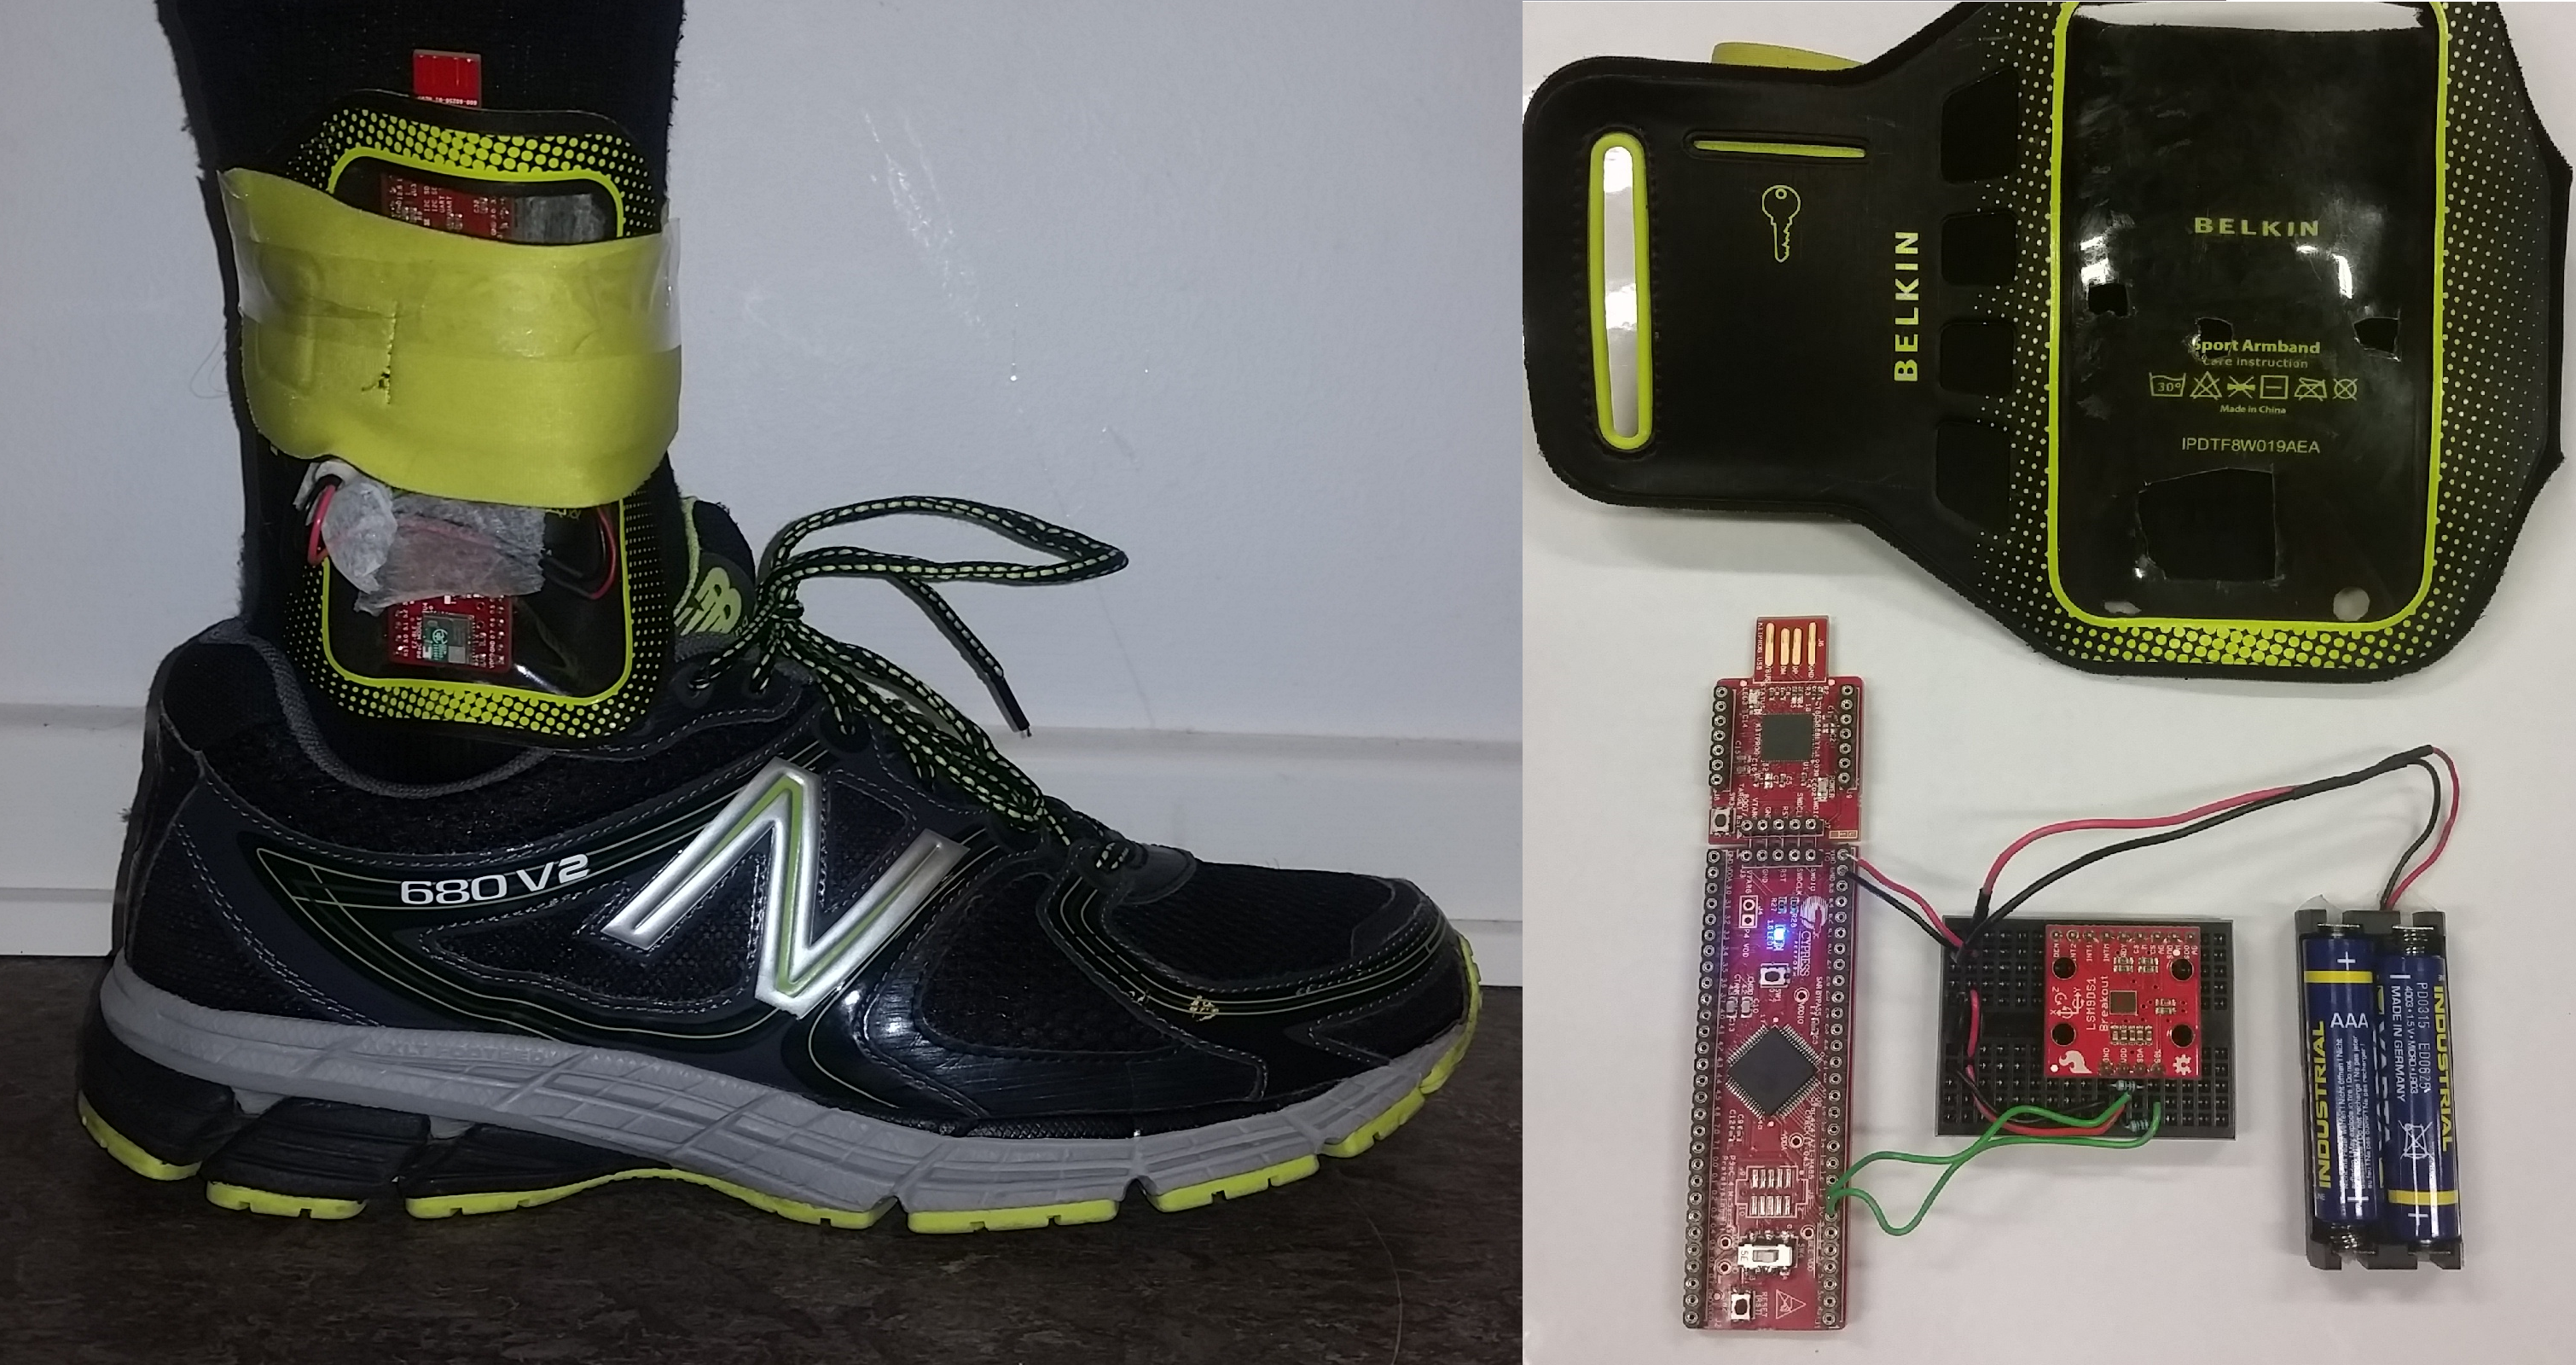
\includegraphics[scale=0.143]{figures/cDesign/samlet_system_paafod3.png}
	\caption{På figuren ses henholdsvis opsætningen af det endelige system på en forsøgsperson samt det samlede system taget ud fra opsætningen. Der ses, at EZ\_BLE modulet er frit tilgængeligt i bunden båndet til venstre i selve opsætningen.}
	\label{fig:samlede_system_opstilling}
\end{figure}

Ved test af det samlede system skal en forsøgsperson udføre tre aktiviteter: gang med 4,8 km/t, løb med 11,3 km/t og cykling med 20,9 km/t. Hver aktivitet skal udføres i 60 sekunder, og dataopsamlingen skal påbegyndes, når forsøgspersonen vurderer at have en homogen cyklus. Forinden tages en 60 sekunders måling, hvor forsøgspersonen står stille på løbebåndet. Det antages, at GUIen herved ikke vil optage nogen aktivitet. Fremgangsmåden for første test af systemet med gang ses herunder: 
\begin{itemize}
	\item GAP central og peripheral skal opdateres med korrekt algoritme på begge 4200M og EZ\_BLE mikroprocessorer.
	\item GAP peripheral med IC og en spændingsforsyning skal placeres proximalt for den laterale malleolus.
	\item GAP central kobles til en PC. 
	\item Forsøgspersonen skal stå oprejst med ret ryg, kigge ligeud og fødderne placeret parallelt på løbebåndet under 60 sekunders måling uden fysisk aktivitet.
	\item Herefter indstilles løbebåndet til en hastighed på 4,8 km/t. Forsøgspersonen går på løbebåndet indtil en homogen cyklus er opnået.  
	\item Et stopur startes samtidig med GUI, hvorved datastreaming fra GAP peripheral visualiseres på PCen.
	\item Dataopsamlingen skal foregå i 60 sekunder ifølge stopuret, hvorefter der trykkes på Q i MATLAB. Dette fryser figuren, således værdierne ved 60 skunder kan aflæses.
	\item Målingen stoppes.
\end{itemize}
Denne fremgangsmåde gentages to gange, hvor anden test er for detektion af løb og tredje test er for detektion af cykling. Forsøgspersonen dog sidder på en motionscykel under detektion af cykling. Resultatet fra denne test fremkommer som en fordeling af aktiviteter på GUIen, der helst ikke skal opfange aktivitet under målingen med ingen fysisk aktivitet. \\
Resultatet fra de forskellige tests ses i \tabref{tab:samlet_sys_test1}
\begin{table}[H]
	\centering
	\begin{tabular}{cccccc}
			\cellcolor[HTML]{C0C0C0}\begin{tabular}[c]{@{}c@{}} Udført\\aktivitet \end{tabular} & 	\cellcolor[HTML]{C0C0C0} Forsøgsperson & 	\cellcolor[HTML]{C0C0C0}\begin{tabular}[c]{@{}c@{}} Detektion af \\ gang {[}Sek{]} \end{tabular} & 	\cellcolor[HTML]{C0C0C0}\begin{tabular}[c]{@{}c@{}} Detektion af \\ løb {[}Sek{]} \end{tabular} & \cellcolor[HTML]{C0C0C0}\begin{tabular}[c]{@{}c@{}} Detektion af \\ cykling {[}Sek{]} \end{tabular} & \cellcolor[HTML]{C0C0C0}\begin{tabular}[c]{@{}c@{}} Afvigelse\\{[}\%{]} \end{tabular} \\ \hline
        \multirow{5}{*}{Gang}                                                     & 1             & 39,9                                                                                                & 1,1                                                                                              & 0  & 2,76                                                                                                   \\
		& 2             & 40,6                                                                                                & 0                                                                                                & 0   & 0                                                                                                  \\
		& 3             & 39                                                                                                  & 2                                                                                                & 0       & 5,13                                                                                              \\
		& 4             & 39,7                                                                                                & 1,6                                                                                              & 0      & 4,03                                                                                               \\
		& 5             & 40,8                                                                                                & 0                                                                                                & 0      & 0                                                                                               \\ \hline
		\multirow{5}{*}{Løb}                                                      & 1                                                                                                          & 1,2 & 39,9                                                                                             & 0     & 3,01                                                                                                \\
		& 2                                                                                           & 1,8  & 39                                                                                            & 0         & 4,62                                                                                            \\
		& 3                                                                                              & 0    & 40,8                                                                                            & 0      & 0                                                                                               \\
		& 4                                                                                                      & 0,4  & 40,4                                                                                            & 0     & 0,99                                                                                                \\
		& 5                                                                                                    & 0     & 40,6                                                                                           & 0         & 0   \\ \hline
		\multirow{5}{*}{Cykling}     & 1     & 0        & 0     & 40    & 0      \\
		& 2             & 0                                                                                                & 0                                                                                                & 40,1       & 0                                                                                              \\
		& 3             & 0                                                                                                  & 0                                                                                                & 40      & 0                                                                                              \\
		& 4             & 0                                                                                                  & 0                                                                                                & 40    & 0                                                                                                 \\
		& 5             & 0                                                                                                  & 0                                                                                                & 36 & 0   \\ \hline                                                                                                
		\end{tabular}
		\caption{I tabellen ses resultaterne fra de tre tests af det samlede system. Derudover er afvigelsen for hver detektion af fysisk aktivitet blevet udregnet.}
		\label{tab:samlet_sys_test1}
\end{table}{-0.5cm}
Der ses i \tabref{tab:samlet_sys_test1}, at GUIen optager mest gangsignal under gang, mest løbesignal under løb og udelukkende signal for cykling, når forsøgspersonen cyklede. Det fremgår ikke af tabellen, men for hver forsøgsperson ved stilstående måling blev der ikke detekteret nogen aktivitet af GUIen. \\
Den største afvigelse i detektion af den bestemte aktivitet er på 5,13\%. Dermed overholder systemet kravet om, at der må være en maks afvigelse på 10\%. Der ses dog også i \tabref{tab:samlet_sys_test1}, at GUIen detekterer cirka 40 sekunders data $pm$1 sekund, selvom dataopsamlingen varer i 60 sekunder. Dette vurderes imidlertid ikke være en faktor, der gør, at systemet vurderes til at være ikke funktionel, da samtlige krav undtagen pulsdetektering opfyldes. Årsagen til at systemet tilsyndeladende ikke sampler en tredjedel af signalet vil blive forklaret og diskuteret i \secref{sec:diskussion}.

Der foretages yderligere en test af systemet, hvor forsøgspersonerne først skal forsøge at gå ved en bestemt hastighed og derefter løbe ved samme hastighed. Derved testes systemet ved en hastighed, som både kan være gang og løb for at undersøge dets reaktion herfra. Fremgangsmåden for dette forsøg fremgår herunder:
\begin{itemize}
	\item GAP central og peripheral skal opdateres med korrekt algoritme på begge 4200M og EZ\_BLE mikroprocessorer.
	\item GAP peripheral med IC og en spændingsforsyning skal placeres proximalt for den laterale malleolus.
	\item GAP central kobles til en PC. 
	\item Forsøgspersonen skal forsøge at gå på løbebåndet med 8 km/t. 
	\item Når en homogen cyklus er opnået, startes et stopur samtidig med GUI, hvorved datastreaming fra GAP peripheral visualiseres på PCen.
	\item Dataopsamlingen skal foregå i 60 ifølge stopuret, hvorefter der trykkes på Q i MATLAB. Dette fryser figuren, således værdierne ved 60 sekunder kan aflæses.
	\item Målingen stoppes.
\end{itemize}
Denne fremgangsmåde testes yderligere, hvor forsøgspersonen skal løbe ved samme hastighed. 8 km/t er valgt på baggrund af pilotforsøget samt litteratur. I pilotforsøget skiftede hver forsøgsperson fra gang til løb under hastighedsstigningen mellem 8 og 20 km/t. Derudover hævder litteratur, at 4 miles per hour (mph) svarer til rask gang mens 6 mph er langsomt løb. 5 mph er cirka 8 km/t, hvilket understøtter valget af hastigheden. \citep{Miles2007} Resultatet fra denne test ses i \tabref{tab:samletsys_8kmt}
\begin{table}[H]
	\centering
	\begin{tabular}{cccccc}
		\cellcolor[HTML]{C0C0C0}\begin{tabular}[c]{@{}c@{}} Udført aktivitet \\ med 8 km/t\end{tabular} & 	\cellcolor[HTML]{C0C0C0} Forsøgsperson & 	\cellcolor[HTML]{C0C0C0}\begin{tabular}[c]{@{}c@{}} Detektion af \\ gang {[}Sek{]} \end{tabular} & 	\cellcolor[HTML]{C0C0C0}\begin{tabular}[c]{@{}c@{}} Detektion af \\ løb {[}Sek{]} \end{tabular} & \cellcolor[HTML]{C0C0C0}\begin{tabular}[c]{@{}c@{}} Detektion af \\ cykling {[}Sek{]} \end{tabular} & \cellcolor[HTML]{C0C0C0}\begin{tabular}[c]{@{}c@{}} Afvigelse\\{[}\%{]} \end{tabular} \\ \hline 
		\multirow{5}{*}{Gang}                                                     & 1             & 36,3                                                                                                & 4,3                                                                                              & 0  & 11,85                                                                                                   \\
		& 2             & 31,1                                                                                                & 9,9                                                                                                & 0   & 31,83                                                                                                  \\
		& 3             & 2,3                                                                                                  & 38,3                                                                                                & 0       & 94,3                                                                                              \\
		& 4             & 4                                                                                                & 36,7                                                                                              & 0      & 90,17                                                                                               \\
		& 5             & 0,4                                                                                                & 40,4                                                                                                & 0      & 99,02                                                                                               \\ \hline
		\multirow{5}{*}{Løb}                                                      & 1                                                                                                          & 0,8 & 40                                                                                             & 0     & 2                                                                                                \\
		& 2                                                                                           & 0,9  & 40                                                                                            & 0         & 2,25                                                                                            \\
		& 3                                                                                              & 2,3    & 38,6                                                                                            & 0      & 5,96                                                                                               \\
		& 4                                                                                                      & 0,2  & 40,7                                                                                            & 0     & 0,49                                                                                                \\
		& 5                                                                                                    & 0,9     & 40,2                                                                                           & 0         & 2,24   \\ \hline 
		\end{tabular}
	\caption{I tabellen ses resultaterne fra en test, hvor forsøgspersonerne skulle henholdsvis gå eller løbe ved samme hastighed. Der ses yderligere, at afvigelserne ved en mellemting mellem gang og løb er betydeligt mere signifikante, end ved klar gang eller løb. Dette går især ud over detektering af aktiviteten gang.}
	\label{tab:samletsys_8kmt}
\end{table}{-0.5cm}
Der ses i \tabref{tab:samletsys_8kmt}, at når tempoet for aktiviteten ikke er klar gang eller løb for forsøgspersonen, så vil den procentvise fordeling stige meget drastisk for gang data. Dette grunder i, at 8 km/t vurderes som værende meget rask gang fra hver forsøgsperson. Derfor vil g påvirkningen af accelerometerets y akse også blive påvirket med mere kræft end ved langsom gang. Der ses, at forsøgsperson 1 og 2 har lavere afvigelse for gangsignalet end forsøgsperson 3 til 5. Dette kan skyldes, at forsøgsperson 1 og 2 er mænd mens 3 til 5 er kvinder, hvor mændene er højere end kvinderne, har derved længere ben og muligvis en anden gangart end kvinderne. Dette diskuteres ligeledes i \secref{sec:diskussion}.

Afslutningsvis testes spændingsforbruget af den eksterne spændingsforsyning, som beskrevet i \secref{spaendingsforsyning}. Dette gøres nu, da en test heraf kræver, at systemet er samlet og under brug for at give en mere realistisk måling. Testen foregik således, at den eksterne spændingsforsyning fik udskiftet batterier og herefter målt outputspændingsniveauet. Efterfølgende blev spændingsforbruget målt hver halve time under samlet systemtest. Der antages, at spændingsforbruget er lineært faldende, hvorfor en gennemsnitsværdi for forbrug per time udregnes. \\
Spændingsforsyningen leverede 3,19 V fra starten af testen. Resultatet af de efterfølgende fem målinger ses i \tabref{tab:samlet_sys_batteri}
\begin{table}[H]
	\centering
	\begin{tabular}{cccc}
		\hline
		\cellcolor[HTML]{C0C0C0}Måling & \cellcolor[HTML]{C0C0C0}\begin{tabular}[c]{@{}c@{}} Spændingsniveau 1 time\\ inden måling {[}V{]} \end{tabular} & \cellcolor[HTML]{C0C0C0}\begin{tabular}[c]{@{}c@{}} Nuværende \\ spændingsniveau {[}V{]} \end{tabular} & \cellcolor[HTML]{C0C0C0}Spændingsforbrug {[}V{]} \\ \hline
		1 & 3,19 & 3,104 & 0,086 \\ \hline	
		2 & 3,104 & 3,052 & 0,052 \\ \hline	
		3 & 3,052 & 3,016 & 0,036 \\ \hline
		4 & 3,016 & 2,969 & 0,047 \\ \hline
		5 & 2,969 & 2,951 & 0,018 \\ \hline
	\end{tabular}
	\caption{I tabellen ses resultatet fra målingerne af spændingsforbruget for den eksterne spændingsforsyning. Der ses yderligere det beregnede spændingsforbrug for hver måling.}
	\label{tab:samlet_sys_batteri}
\end{table}\vspace{-0.5cm}
I \tabref{tab:samlet_sys_batteri} ses spændingsforbruget over fem målinger med en halv times interval. Da det antages, at spændingsforbruget har et lineært forhold, bliver en gennemsnit beregnet i \eqref{eq:samlet_sys1}
\begin{equation}
\frac{0,086 + 0,052 + 0,036 + 0,047 + 0,018}{5} \cdot 2 = 0,0956~V
\label{eq:samlet_sys1}
\end{equation}
Med antagelse af lineært forhold vil spændingsforsyningen falde med 0,0956 V per time. Da startspændingen var 3,19 V og den endelige spænding, hvormed MCUen ikke længere er funktionel, er 1,71 V, må det maksimale forbrug være $3,19 - 1,71 = 1,48$ V. Derfor er levetiden for den eksterne spændingsforsyning udregnet til:
\begin{equation}
\frac{1,48}{0,0956} = 15,481~timer.
\label{eq:samlet_sys2}
\end{equation}
I \eqref{eq:samlet_sys2} ses det, at den eksterne spændingsforsyning teoretisk kan få det samlede sytem til at være funktionel i 15,481 timer. Derfor overholder det samlede system kravet om, at det skal besidde batterilevetid for en hel dag svarende til 15 timer.
%
%
%\begin{table}[H]
%	\centering
%	\begin{tabular}{ccccc}
%		\hline
%		\rowcolor[HTML]{C0C0C0} 
%		Udført aktivitet & \begin{tabular}[c]{@{}c@{}} Detektion \\ af gang {[}Min{[} \end{tabular} & \begin{tabular}[c]{@{}c@{}} Detektion\\ af løb {[}Min{[}\end{tabular} & \begin{tabular}[c]{@{}c@{}} Detektion \\ af cykling {[}Min{[}\end{tabular} & y \\ \hline
%		Gang & 0 & 100 & 0 & 100 \\ \hline
%		Løb & 0 & 100 & 0 & 0 \\ \hline
%		Cykling & 0 & 0 & 100 & 0 \\ \hline
%	\end{tabular}%
%\end{table}\vspace{-.5cm}
%
%Der ses i \tabref{tab:samlet_sys_test1}, at systemet ikke detekterer gang korrekt. Det antages at være i forbindelse med tærskelværdierne, der adskiller gang og løb. Data fra Shimmer skal multipliceres med 16 for at give samme output, som data fra ICen, hvilket fremgår i \secref{sec:algogangloeb}. Der findes dog ikke samme forhold efter databehandlingen, hvorfor tærskelværdierne ikke blot kan multipliceres med 16. Derfor fortages endnu test, hvor målingerne skal ske ved konstant hastighed for henholdsvis gang og løb for at undersøge maksimal peak værdier. Derudover skal GAP peripheral kun sende data fra accelerometret, hvilket visualiseres i Realterm ved hjælp af GAP central. Algoritmen på GAB peripheral reguleres altså således, at gyroskopets data ikke sendes via BLE og tidsenheden imellem maks peaks er i dette tilfælde relevant. Der ønskes udelukkende en værdi for detekteringen af maks peak. Fremgangsmåden for denne test forekommer således:
%\begin{itemize}
%		\item GAP central og peripheral skal opdateres med korrekt algoritme på begge 4200M og EZ\_BLE mikroprocessorer.
%		\item GAP peripheral med IC og en spændingsforsyning skal placeres proximalt for den laterale malleolus.
%		\item GAP central kobles til en PC. 
%		\item En test af forbindelsen imellem GAP central og peripheral testes ved brug af Realterm på PCen.
%		\item Løbebåndet indstilles til 4,8 km/t. Forsøgspersonen går på løbebåndet indtil en konstant hastighed er opnået.
%		\item Realterm skal herefter visualisere data i 30 .
%		\item Målingen stoppes
%\end{itemize}
%Samme test fortages, hvor løbebåndet indstilles til 11,3 km/t. Data fra realterm konverteres, således Matlab kan genkende datatypen, hvorved en gennemsnitsværdi beregnes. Resultatet af disse to tests ses i \tabref{tab:samlet_sys_regulering}
%\begin{table}[H]
%	\centering
%	\begin{tabular}{cc}
%		\hline
%		\rowcolor[HTML]{C0C0C0} 
%		Aktivitet & \begin{tabular}[c]{@{}c@{}} Gennemsnitsværdi \\ for maks peak \end{tabular} \\ \hline
%			Gang & ? \\ \hline
%			Løb & ? \\ \hline
%		\end{tabular}%
%		\caption{I tabellen ses resultatet fra reguleringstesten for accelerometerdata.}
%		\label{tab:samlet_sys_regulering}
%\end{table}\vspace{-.5cm}
%Der ses i \tabref{tab:samlet_sys_regulering}, at maks peak værdierne for gang er langt højere, end værdierne var ved brug af Shimmer sensoren. Tærskelværdien for gang er 50, mens den for løb er 400. Disse skal reguleres, hvorefter det antages at algoritmen er tilpasset ICen. Ud fra værdierne fra \tabref{tab:samlet_sys_regulering} vælges de regulerede tærskelværdier til henholdsvis ? og ?. De nye tærskelværdier fremgår i \tabref{tab:samlet_sys_regulering2}.
%\begin{table}[H]
%	\centering
%	\begin{tabular}{ccc}
%		\hline
%		\rowcolor[HTML]{C0C0C0} 
%		Aktivitet & Gammel tærskelværdi & Reguleret tærskelværdi \\ \hline
%		Ingen aktivitet &  x~$\textless$~50 & ? \\ \hline
%		Gang & 50~$\textless$~x~$\textgreater$~400 & ? \\ \hline
%		Løb & 400~$\textgreater$~x & ? \\ \hline
%	\end{tabular}%
%	\caption{I tabellen ses resultatet fra reguleringstesten for accelerometerdata.}
%	\label{tab:samlet_sys_regulering2}
%\end{table}\vspace{-.5cm}
%Dette korrigeres inde i algoritmedesignet. Herefter fortages de tre seperate tests igen for det samlede system. Resultatet heraf ses i \tabref{tab:samlet_sys_test2}.
%\begin{table}[H]
%	\centering
%	\begin{tabular}{ccccc}
%		\hline
%		\rowcolor[HTML]{C0C0C0} 
%		Test nummer & \begin{tabular}[c]{@{}c@{}} Detektion \\ af gang {[}\%{[} \end{tabular} & \begin{tabular}[c]{@{}c@{}} Detektion\\ af løb {[}\%{[}\end{tabular} & \begin{tabular}[c]{@{}c@{}} Detektion \\ af cykling {[}\%{[}\end{tabular} & \begin{tabular}[c]{@{}c@{}} Afvigelse {[}\%{[} \end{tabular} \\ \hline
%			1 & 100 & 0 & 0 & 0 \\ \hline
%			2 & 0 & 100 & 0 & 0 \\ \hline
%			3 & 0 & 0 & 100 & 0 \\ \hline
%		\end{tabular}%
%		\caption{I tabellen ses resultaterne fra de tre tests af den anden samlede test af systemet. Der ses, at detektionen af den specifikke aktivitet er mere præcis efter reguleringen af tærskelværdierne.}%mhandlede revurdering af algoritmens tærskelværdier, samt vurdering af pulssensor.}
%		\label{tab:samlet_sys_test2}
%\end{table}\vspace{-.5cm}
%Det ses i \tabref{tab:samlet_sys_test2}, at systemet overholder kravet om en maksimal afvigelse på 10\% i forhold til fejlvurdering af aktivitet. \textbf{kog noget mere på det her, når vi har testet}.
%
%Systemet testes ligeledes for batteriets levetid. %, med henblik på at af,- eller bekræfte kravet vedrørende at kunne være batteridrevet igennem en hel dag. 
%Systemets initialeres til at starte samtidig med et stopur. Det samlede systems spændingsforsyning tilkobles et multimeter for at kunne måle dets spænding inden forsøget. Systemet skal køre uafbrudt i en time, hvorefter spændingsforsyningens igen tilkoples et multimeter og måles igen. 
%\begin{table}[H]
%	\centering
%	\begin{tabular}{cc}
%		\hline
%		\rowcolor[HTML]{C0C0C0} 
%		Spændingsniveau før forsøg {[}V{]} & Spændingsniveau efter forsøg {[}V{]} \\ \hline
%		3,14 & ????2,78???? \\ \hline
%	\end{tabular}
%	\caption{I tabellen ses testresultaterne vedrørende det samlede systems spændingsforbrug.}
%	\label{tab:test_spaending}
%\end{table} \vspace{-.5cm}
%Ud fra ovenstående testresultater beregnes der, at det samledes system forbruger 0,36 V per time. På baggrund i design af sensoren LSM9DS1 vides der, at den minimale tilførte spænding for funktionalitet af sensoren er 2,40 V. Dette resulterer systemet kan forbruge 0,74 V fra start, hvorefter systemet ikke forventes at fungere mere. 
%
%\begin{equation}
%Varighed~vedr\text{ø}rende~line\text{æ}r~operation = \frac{0,74~V}{0,36~V~per~time} = 2,05~timer
%\end{equation}   
%Det samlede system vil efter 2,05 timer have opbrugt tilpas spænding, således sensoren ikke længere er funktionel. % have opbrugt det spændingsarbejdsområde, hvoraf sensoreren opererer lineært. 
%Test af systemets levetid per batteri afkræfter dermed kravet heraf.
%
%Det samlede systems krav vedrørende et komfortabelt produkt for brugeren, samt bestå af et motiverende element for børn i aldersgruppen 9-12 år, blev ikke implementeret. Dette blev ikke implementeret, da systemet er en prototype, hvoraf fokus er på dets funktionalitet.  